%\newpage

\newcommand{\KSll}{B^0\to K^* \ell^+\ell^-}
\newcommand{\KSmm}{B^0\to K^* \mu^+\mu^-}
\newcommand{\KSee}{B^0\to K^* e^+e^-}
\newcommand{\Kll}{B^{\pm}\to K^{\pm} \ell^+\ell^-}
\newcommand{\Kmm}{B^{\pm}\to K^{\pm} \mu^+\mu^-}
\newcommand{\Kee}{B^{\pm}\to K^{\pm} e^+e^-}
\newcommand{\pt}{p_\mathrm{T}}
\newcommand{\acc}{\mathcal{A}}
\newcommand{\eff}{\epsilon}
\newcommand{\ate}{\acc\eff}
\newcommand{\jpsi}{\mathrm{J/}\psi}
\newcommand{\jpsill}{\jpsi\to\ell\ell}
\newcommand{\jpsiee}{\jpsi\to\mathrm{ee}}
\newcommand{\jpsimm}{\jpsi\to\mu\mu}
\newcommand{\zmm}{\mathrm{Z}\to\mu\mu}
\newcommand{\TeV}{\rm{TeV}}
\newcommand{\conv}{\gamma\to\mathrm{ee}}
\newcommand{\bincl}{B_\mathrm{tag}\to\mu_\mathrm{tag}\mathrm{X}}
\newcommand{\bsig}{B_\mathrm{sig}{\to}K^{(*)}\ell\ell}
\newcommand{\bksig}{B^{\pm}_\mathrm{sig}{\to}K^{\pm}\ell\ell}
\newcommand{\bkstsig}{B^{0}_\mathrm{sig}{\to}K^{*0}\ell\ell}

\section{Low-momentum electron reconstruction}
\label{electron}

One of the most crucial experimental aspects of the $R_{K^{(*)}}$
measurements is the ability to identify low-$\pt$ electrons down to
$\pt \gtrsim 1~\GeV$. The following subsections outline the
performance limitations of the current electron reconstruction
algorithms, the consequences for the $R_{K^{(*)}}$ measurements, the
proposed strategy for improvements, the primary datasets and simulated
event samples and/or skims required to tune and commission the updated
algorithms, and computing considerations.

%\subsection{Overview of the electron reconstruction chain}
%Single paragraph summary highlighting key aspects and references. 

\subsection{Nominal performance and consequences for the
  \texorpdfstring{$R_{K^{(*)}}$}{RK} measurements} 

Studies based on the simulated pair production of charged B hadrons,
one of which is decayed inclusively (``tag-side'') and the other is
forced to decay via $\Kll$ (``signal-side''), demonstrate that the
acceptance times efficiency $\ate$ obtained with the current electron
reconstuction algorithm severely limits the ability to accurately
measure $R_{K^{(*)}}$.

Figure~\ref{fig:ele_acc_x_eff} (Left) shows the generator-level $\pt$
distributions for the daughter particles from the $\Kll$ decay. The
$\pt$ distributions are very soft, with those for the kaon and
subleading lepton peaking at
${\approx}1~\GeV$. Figure~\ref{fig:ele_acc_x_eff} (Right) shows the
efficiency to reconstruct electrons as a function of the
generator-level $\pt$, as obtained with the default electron
reconstruction algorithm. The efficiency is determined to be
essentially zero for the region $0 < \pt < 2~\GeV$ because of explicit
thresholds applied during the early seeding steps. The efficency is in
the range 0.2--0.8 for the region $2 < \pt < 7~\GeV$, beyond which the
plateau is reached.

\begin{figure}[!h]
  \centering
  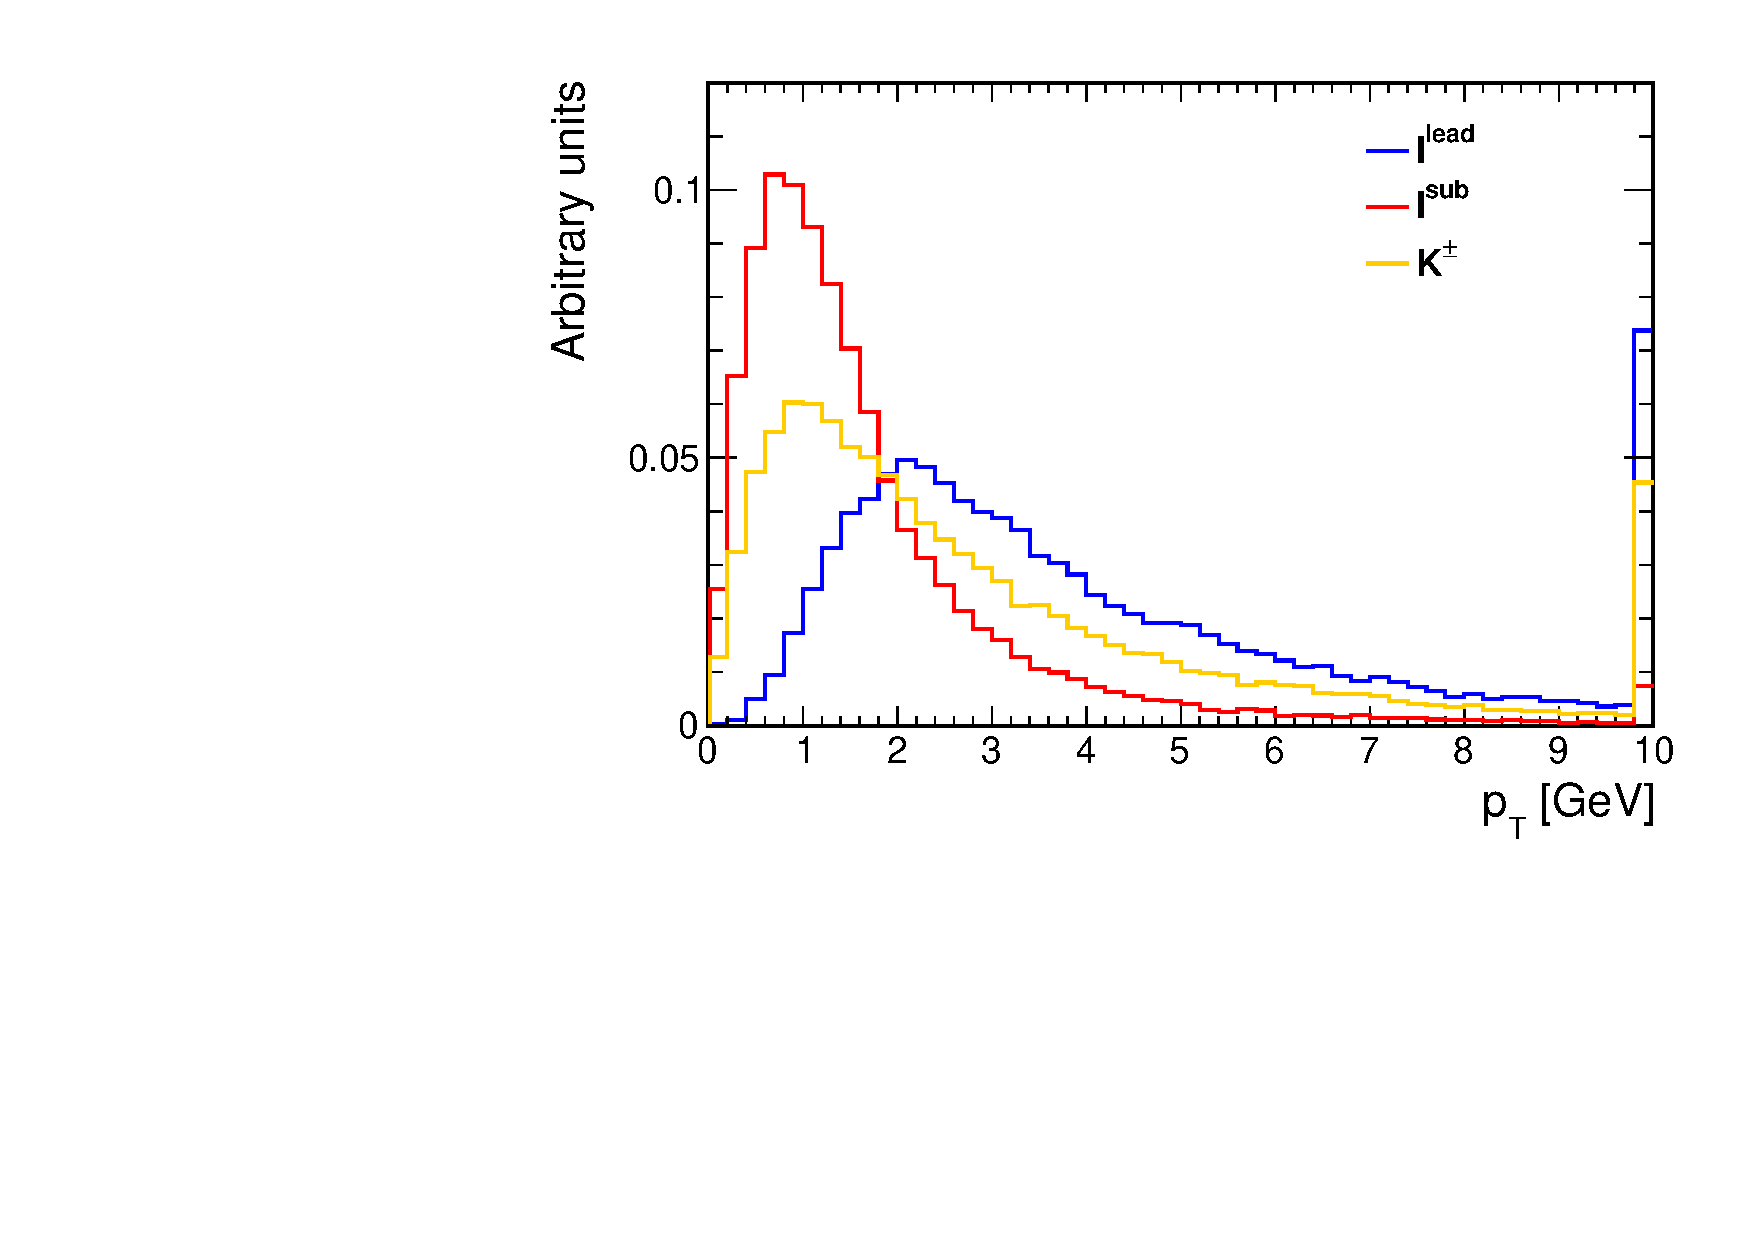
\includegraphics[width=0.48\textwidth]{figures/BKLL_acc.pdf} ~
  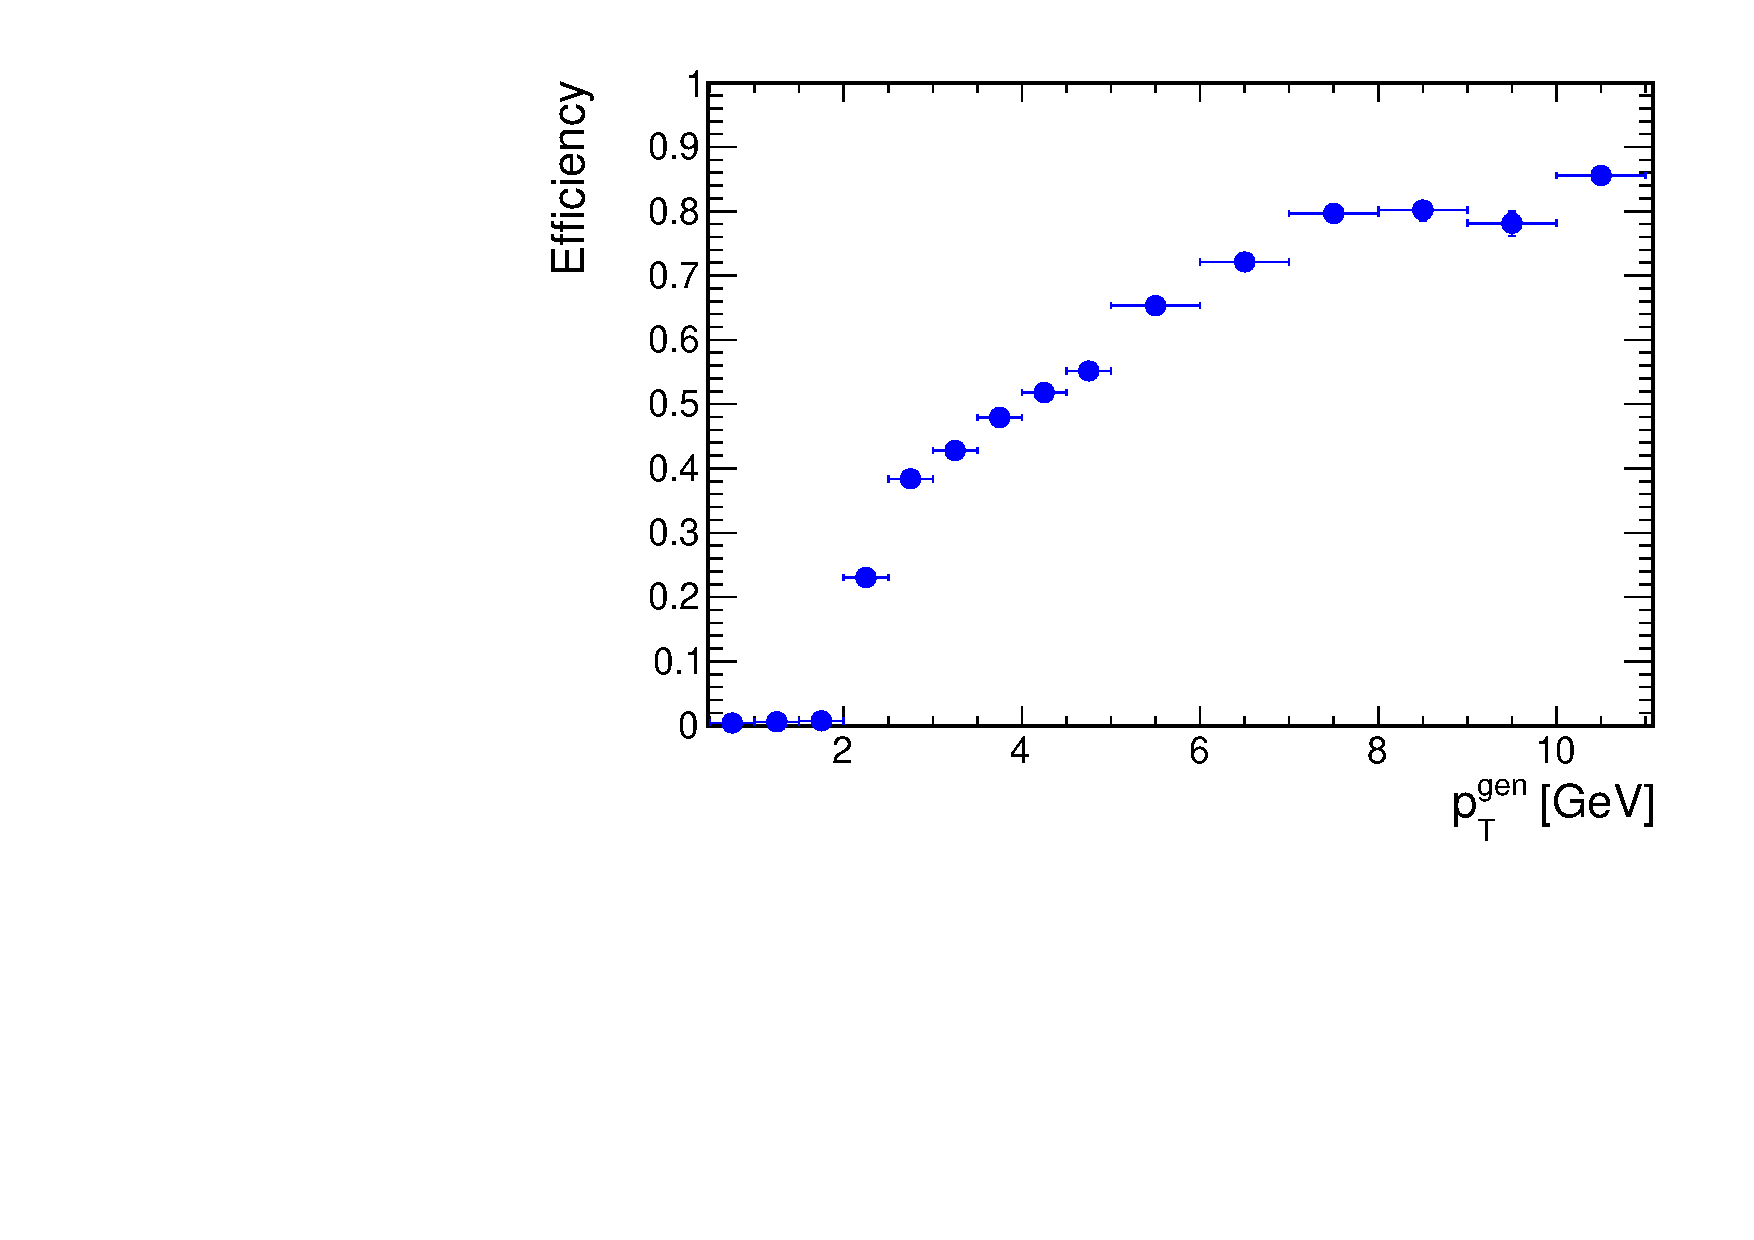
\includegraphics[width=0.48\textwidth]{figures/BKLL_eff.pdf} \\
  \caption{\it (Left) Normalised distributions of the generator-level
    $\pt$ for the daughter particles from the $\Kll$ decay; namely the
    kaon ($K^\pm$), and the leading ($\ell^\mathrm{lead}$) and
    subleading ($\ell^\mathrm{sub}$) leptons. 
    (Right) Efficiency to reconstruct electrons as a function of the
    generator-level $\pt$, as obtained with the default electron
    reconstruction algorithm.  
%    (Right) Efficiency to reconstruct kaons ($K^\pm$) and the leading
%    ($e^\mathrm{lead}$) and subleading ($e^\mathrm{lead}$) electrons
%    as a function of the $\pt$ of the matched generator-level object,
%    obtained with the default reconstruction algorithms.
  \label{fig:ele_acc_x_eff}}
\end{figure}

Table~\ref{tab:ele_acc_x_eff} shows both the $\acc$ values for both
$\Kll$ and $\KSll$ decays, as well as the $\ate$ values for both
$\Kee$ and $\KSee$ decays, for a set of minimum tranverse momentum
requirements, $\pt^\mathrm{min}$, applied to both daughter leptons,
while considering a fixed $\pt$ requirement for the kaon ($\pt >
0.5~\GeV$). The requirement $|\eta| < 2.5$ is applied to all daughter
particles. The $\acc$ values are comparable for $\Kll$ and $\KSll$ and
depend strongly on the transverse momentum threshold
$\pt^\mathrm{min}$. Acceptances of 8--11\% can be raised to 27--44\%
by reducing $\pt^\mathrm{min}$ from the default value of $2~\GeV$ to
$0.7~\GeV$ (the latter threshold is the minimum $\pt$ required for an
electron to reach the ECAL barrel). When folding in the electron
reconstruction efficiencies, the $\ate$ values increase slowly with
decreasing $\pt^\mathrm{min}$ and do not exceed ${\approx}5\%$ below
$2~\GeV$ with the current electron reconstruction algorithm. However,
a factor 2--5 increase in $\ate$ can be achieved with even moderate
improvements in efficiencies when combined with the lowering of
$\pt^\mathrm{min}$.

\begin{table}[!h]
  \footnotesize
  \center
  \caption{\it The $\acc$ values for both $\Kll$ and $\KSll$ decays,
    as well as the $\ate$ values for both $\Kee$ and $\KSee$ decays,
    for a set of minimum tranverse momentum requirements,
    $\pt^\mathrm{min}$, applied to both daughter leptons, while
    considering a fixed $\pt$ requirement for the kaon ($\pt >
    0.5~\GeV$). The requirement $|\eta| < 2.5$ is applied to all
    daughter particles. \label{tab:ele_acc_x_eff}}
  \vspace{0.1in}
  \begin{tabular}{ cccccc }
    \hline
    $\pt^\mathrm{min}$ & \multicolumn{2}{c}{$\acc$} &         & \multicolumn{2}{c}{$\ate$} \\
    \cline{2-3}\cline{5-6} 
    [GeV]              & $\Kll$                     & $\KSll$ &  & $\Kee$ & $\KSee$        \\
    \hline                                
    5.0                & 0.02                       & 0.02    &  & 0.01   & 0.01           \\ 
    2.0                & 0.11                       & 0.08    &  & 0.05   & 0.04           \\ 
    1.0                & 0.32                       & 0.19    &  & 0.05   & 0.04           \\ 
    0.7                & 0.44                       & 0.27    &  & 0.05   & 0.04           \\ 
    \hline
  \end{tabular}
\end{table}

\subsection{Baseline strategy for improving
  \texorpdfstring{$\ate$}{AxE}}
\label{sec:strategy}

Significant improvements in $\ate$ are possible, with minimal
intervention, through the reoptimisation of existing thresholds and
parameters used in the reconstruction chain. This statement is
supported by experts within the EGM POG and is based on the fact that
the current ``tracker-driven'' algorithm does not fully exploit the
tracking performance in the very low $\pt$ regime and, further,
several parameters and multivariate techniques have not been tuned to
reflect changes in the LHC beam parameters and detector configuration
betweens LHC Runs 1 and 2. 

Studies are already underway to explore possible performance gains at
the tracker-driven seeding step, which involve the consideration of
low-$\pt$ tracks (i.e. below $2~\GeV$) as inputs to the seeding step,
as well as the retraining of a BDT that improves efficiencies in the
region $2 < \pt < 50~\GeV$ (and potentially below). Similar studies
are expected at later stages in the electron reconstruction
chain. Further, the electron identification criteria will also be
revisited for the low-$\pt$ regime. Finally, more involved studies and
developments may be used if deemed necessary, although our baseline
strategy is to minimise intervention. All studies are being carried
out in close collaboration with the EGM POG community.

%First pass: \\
%- Minimal intervention, no changes to reconstruction chain, simple ``tuning''.\\
%- Tuning of existing configurable thresholds?\\
%- e.g. lowering track pT related thresholds at the seeding (and later?) stages.\\
%- Retraining the BDTs at the seeding (and later?) stages for Run 2 conditions.\\
%Second pass (need to be careful here):\\
%- Optimisation of the BDTs?\\
%- Tweaks to reconstruction?\\
%- Other?\\

\subsection{Commissioning of low-\texorpdfstring{$\pt$}{pT} electrons}

The following subsections outline a minimal set of primary datasets
and simulated event samples that can be used to optimise the electron
reconstruction and identification algorithms, measure reconstruction
and identification efficiencies, and determine the associated
data-to-simulation scale factors.
%The required primary datasets and simulated samples are summarised in
%Table~\ref{tab:samples}.

%\begin{table}[!h]
%  \footnotesize
%  \center
%  \caption{\it  \label{tab:samples}}
%  \vspace{0.1in}
%  \begin{tabular}{ lllll }
%    \hline
%    PD or simulated sample & Topology & Data tier & Scope & Sample
%    size \\
%    \hline
%    \verb!SingleElectron! & $\conv$ convs. & \verb!RAW! &
%    RECO, ID optimisation & Skim of ${\approx}1~\ifb$ \\
%    \verb!DoubleMuon! & $\jpsiee$ (PU) & \verb!RAW! &
%    RECO, ID optimisation & Skim of ${\approx}1~\ifb$ \vspace{0.1cm} \\
%    \verb!SingleElectron! & $\conv$ convs. & \verb!MiniAOD!
%    & Efficiencies, SFs & 2017 dataset \\
%    \verb!DoubleMuon! & $\jpsiee$ (PU) & \verb!MiniAOD! &
%    Efficiencies, SFs & 2017 dataset \\
%    $\bincl$, $\bsig$ & $\jpsiee$ (PU) & \verb!MiniAOD! &
%    Efficiencies, SFs & 2017 dataset \\
%    \hline
%  \end{tabular}
%\end{table}


\subsubsection{Simulated samples}
\label{sec:simulated_samples}

Optimisation and efficiency studies are ongoing, based on the
following privately produced samples:
%\begin{itemize}
%\item
charged B meson pair production, with $\bincl$ and $\bksig$, with
$\ell = \mathrm{e}, \mu$ and $\pt(\mu_\mathrm{tag}) > 7~\GeV$;
%\item
neutral B meson pair production, with $\bincl$ and $\bkstsig$, with
$\ell = \mathrm{e}, \mu$ and $\pt(\mu_\mathrm{tag}) > 5~\GeV$.
%\end{itemize}
Samples for the prompt and nonprompt production of $\jpsill$ may also
be produced.

\subsubsection{Data sample of asymmetric
  \texorpdfstring{$\conv$}{conversion} events}

A large sample of low-$\pt$ electrons can be obtained from converted
photons resulting from interactions with the beam pipe and inner
tracking structures. A collection of \verb!reco::Conversion! objects
is available in the \verb!AOD! data tier, the production of which is
based on the following inputs: the ``general'' and ``conversion''
\verb!reco::Track!  collections, the latter of which produced using
dedicated steps that supplement the default tracking sequences; and
the ``ECAL- and tracker-driven'' \verb!reco::GsfElectrons!
collections.

Preliminary studies demonstrate that a large, relatively pure sample
$\conv$ events that contain a low-$\pt$ electron, in the range
1--20~$\GeV$, can be obtained through a minimal set of selection
criteria comprising the presence of an leading electron with $\pt >
20~\GeV$ and a two-track vertex consistent with the conversion
topology. An analysis of $0.6~\ifb$ of data from 2017 era F of the
\verb!SingleElectron! primary dataset yields ${\approx}5 \times 10^4$
low-$\pt$ conversions, with ${\approx}3 \times 10^4$ events satisfying
a tighter $\pt$ requirement on the leading electron as well as the
trigger requirement \texttt{HLT\_Ele32\_WPTight\_Gsf OR
  HLT\_Ele27\_WPTight\_Gsf}. The \verb!RAW! data tier for this sample
is now available on disk and is being used to tune the reconstruction
of low-$\pt$ electrons.

%Reasonable signal to noise, clear view of the pixel detector
%No beampipe shown, due to a preselection in the conversions (AOD)
%~16k in the first layer of the pixel barrel 
%Tune the conversions to include the beam pipe and produce and unbiased1 dataset.

\subsubsection{An unbiased data sample of
  \texorpdfstring{$\jpsiee$}{J/psi} events}
\label{sec:jpsi_from_pu_sample}

A large unbiased sample of $\jpsiee$ events can be obtained from the
2017 dataset by relying on $\jpsi$ production from pileup events. The
cross section times branching fraction $\sigma_{\jpsi}
\mathcal{B}(\jpsimm)$, over the range $6.5 < \pt(\jpsi) < 30~\GeV$ and
$|y(\jpsi)| < 2.4$, is ${\approx}100~\mathrm{nb}$ at $\sqrt{s} =
7~\TeV$~\cite{Khachatryan:2010yr}. The $\sigma\mathcal{B}$ is assumed
to scale to ${\approx}1000~\textrm{nb}$ for $\pt(\jpsi) > 3~\GeV$
(Fig.~3~\cite{Khachatryan:2010yr}). A further factor two increase is
assumed to account for the parton luminosity ratio between $\sqrt{s} =
7$ and $13~\TeV$. Hence the number $\mathcal{N}$ of $\jpsi(\to ee)$
events available during the 2017 dataset is given by
\begin{equation}
  \begin{split}
    \mathcal{N} = &\, R_\mathrm{HLT} \times t_\mathrm{LHC} \times
    n_\mathrm{PU} \times \sigma_{\jpsi}
    \mathcal{B}(\jpsimm) \,/\, \sigma_\mathrm{MB} \\
    = &\, R_\mathrm{HLT}~\mathrm{[Hz]} \times 6 \times
    10^{6}~\mathrm{[s]} \times 38 \times 2~\mathrm{[{\mu}b]} \,/\,
    80~\mathrm{[mb]} \\
    = &\, 5700 \times R_\mathrm{HLT}~\textrm{[Hz]}
  \end{split}
\end{equation}
where $R_\mathrm{HLT}$, $t_\mathrm{LHC}$, $n_\mathrm{PU}$, and
$\sigma_\mathrm{MB}$ are the HLT trigger rate, total live time of the
2017 data-taking period, average number of pileup events, and the
minimum bias cross section, respectively. Estimates for each variable
are given above, and their product yields 5700 $\jpsiee$ events per Hz
of trigger rate.

A skim of events based on the \verb!DoubleMuon! primary dataset could
be used to collect events containing at least one high-$\pt$ muon
(e.g. $\zmm$) that allows the identification of the primary vertex. A
tag-and-probe approach can by used with electron-track pairs that form
a vertex consistent with a pileup interaction and an invariant mass
consistent with the $\jpsi$. The
\verb!HLT_Mu17_TrkIsoVVL_Mu8_TrkIsoVVL_DZ_Mass3p8_v4! trigger and the
\verb!DoubleMuon! PD provide rates of ${\approx}$40 and
${\approx}$100~Hz, respectively, providing a sample of
$\mathcal{O}(10^5)$ events for efficiency measurements. A skim of
$\zmm$ events based on the \verb!RAW! data tier can be used to tune
the reconstruction of low-$\pt$ electrons. Alternatively, the skim for
photon conversions, described above, based on the \verb!RAW! data tier
from the \verb!SingleElectron! primary dataset and the trigger
requirement \texttt{HLT\_Ele32\_WPTight\_Gsf OR
  HLT\_Ele27\_WPTight\_Gsf} could also be used.

%Data and simulation samples for the development and commissioning of
%low-$\pt$ electrons.
%- B pair production with $B_1$ from dimuon trigger and $B_2\to K J$/$\psi$ \\
%- B pair production with 1--5\% of parked dataset and $B_2\to K J$/$\psi$  \\
%- ``tag and probe'' with $J/\psi(\to ee)$ from single electron
%trigger \\
%- ``tag and probe'' with $J/\psi(\to ee)$ from pileup\\
%- $\gamma\to\ ee$ conversions?\\
%- Datasets? Skims? Sample size? Pros/cons of each? 

\subsection{Computing constraints}

\begin{itemize}
\item The tuning of the electron reconstruction and identification
  algorithms will require access to the \verb!RAW! data tier.
\item The studies related to reconstruction and identification of
  low-$\pt$ electrons are expected to take several months and thus the
  integration of algorithm changes into CMSSW are expected to occur
  towards the end of 2018.
\item At a minimum, any developments related to low-$\pt$ electrons
  need only be included in a (patched) CMSSW release dedicated to the
  reconstruction of the parked dataset.
\item The effect of algorithm changes on event size at the
  \verb!RECO!, \verb!AOD!, and \verb!miniAOD! data tiers, as well as
  the additional CPU load, will be assessed in due course. Preliminary
  studies indicate a minimal overhead at the \verb!RECO! data tier.
\item Any high-level analysis that uses low-$\pt$ electrons (e.g. the
  $R_{K^{(*)}}$ measurements) will rely on an ``extended''
  \verb!miniAOD! data tier that contains a \verb!reco::GsfElectron!
  collection (and associated collections) down to
  ${\approx}1~\GeV$.
\end{itemize}

\subsection{Contributions from Imperial}

The contributions from Imperial will focus on improving the $\ate$ to
low-$\pt$ electrons according the strategy outlined in
Sec.~\ref{sec:strategy}, using both simulated samples
(Sec.~\ref{sec:simulated_samples}) and $\jpsiee$ events from pileup
(Sec.~\ref{sec:jpsi_from_pu_sample}).

%Commissioning studies? Data tier? Skims?\\
%Data tier for analysis? ``Extended miniAOD''?\\
%Effect on CPU?\\
%Effect on event size?\\
%Release integration and schedule?\\
%RERECO of parked dataset?\\
%Timelines?

%\newpage
